\chapter{Frequency Response Analysis of a Single Board Heater System by the application of Sine Wave}
The aim of this experiment is to do a Frequency Response Analysis of a Single Board Heater System by the application of Sine Wave.The target group is anyone who has basic knowledge of Control Engineering.
\begin{figure}
\centering
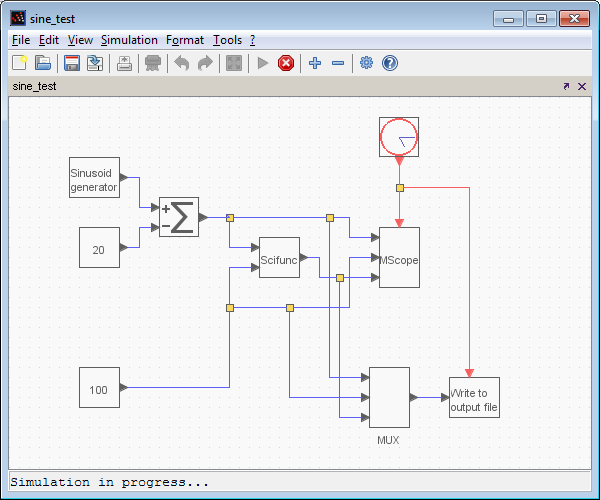
\includegraphics[width=\linewidth]{sinetest_manual/sinetest_xcos.png}
\caption{Xcos for this experiment}
\label{xcos_sine}
\end{figure}
We have used Scilab with Xcos as an interface for sending and receiving data. This interface is shown in Fig.\ref{xcos_sine}. Heater current and Fan speed are the two inputs to the system. The Heater current is varied sinusoidally. A provision is made to set the parameters related to it, like Frequency, Amplitude and Offset. The temperature profile thus obtained is the output.
In this experiment we are applying a sine change in the heater current by keeping the Fan speed constant. After application of sine change, wait for sufficient amount of time to allow the temperature to reach a steady-state.
\section{Theory}
 Frequency Response of a system means its steady-state response to a sinusoidal input. For obtaining a Frequency Response of a system, we vary the frequency of the input signal over a spectrum of interest. The analysis is actually quite useful and also simple because it can be carried out with the available signal generators and measuring devices.
Consider a sinusoidal input
\begin{align}
U(t) &= Asin \omega t
\intertext{The Laplace Transform of the above equation yields}
U(s) &= \frac{A\omega}{s^2 + \omega^2}
\intertext{Consider the standard first order transfer function given below}
G(s) &= \frac {Y(s)}{U(s)} = \frac K{s + 1}
\intertext{Putting the value of U(s) from equation, we get}
Y(s) &= \frac{KA\omega}{(\tau s + 1)(s^2 + \omega ^2)}\\
&=\frac{KA}{\omega ^2\tau ^2 + 1}\left[\frac{\omega \tau ^2}{\tau s +1}- \frac{\tau s \omega}{s^2 + \omega^2}+\frac{\omega}{s^2 + \omega^2}\right]
\intertext{Taking Laplace Inverse, we get}
y(t) &= \left[\frac {KA}{\omega^2\tau^2+ 1}\right]\left[\omega \tau e^{\frac {-t}{\tau}}-\omega \tau cos(\omega t)+sin(\omega t)\right] 
\intertext{The above equation has an exponential term $e^\frac{-t}{\tau}$. Hence, for large value of time, its value will approach to zero and the equation will yield a pure sine wave. One can also use trigonometric identities to make the equation look more simple.}
y(t) &= \left[\frac{KA}{\sqrt{\omega^2 \tau^2 + 1}}\right]\left[sin (\omega t) + \phi \right]
\intertext{where,}
\phi &= -tan^{-1}(\omega \tau)
\intertext{By observing the above equation one can easily make out that for a sinusoidal input the output is also sinusoidal but has some phase difference. 
Also, the amplitude of the output signal, $\hat{A}$, has become a function of the input signal frequency, $\omega$.}
\hat{A}&=\frac{KA}{\sqrt{\omega^2 \tau^2 + 1}}
\intertext{The amplitude ratio (AR) can be calculated by dividing both sides by the input signal amplitude A.}
AR &=\frac{\hat{A}}{A}=\frac{K}{\sqrt{\omega^2 \tau^2 + 1}}
\intertext{Dividing the above equation by the process gain K yields the normalized amplitude ratio $(AR_n)$}
AR_n &=\frac{AR}{K}=\frac{1}{\sqrt{\omega^2 \tau^2 + 1}}
\intertext{Because the process steady state gain is constant, the normalized amplitude ratio often is used for frequency response analysis.\cite{dale04}}
\end{align}

\section{Step by step procedure to perform Sine Test}
Change the current working directory of scilab to the folder {\tt Sine\_Test}. Execute the code {\tt ser\_init.sce} and {\tt sine\_test.sci}. Open the Xcos code {\tt sine\_test.xcos}. Initiate a sine input to the system by setting Sinusoid generator block properties with some value of the frequency  (here $0.007Hz$) and amplitude(hear 10). Note that at high frequencies the plant output is not sinusoidal,which is not of any use. Hence,avoid choosing frequencies above $0.04Hz$.

\begin{figure}
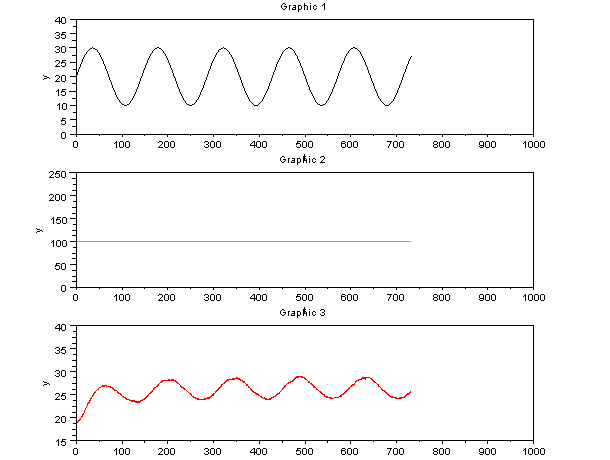
\includegraphics[width=\linewidth]{sinetest_manual/sine_resp.png}
\caption{Plot for sine input 0.007Hz}
\label{fig:scope}
\end{figure}
\begin{table}

\begin{verbatim}
 0.100E+00  0.200E+02  0.100E+03  0.239E+02
 0.200E+00  0.201E+02  0.100E+03  0.238E+02
 0.300E+00  0.201E+02  0.100E+03  0.238E+02
.
.
.
 0.749E+03  0.300E+02  0.100E+03  0.301E+02
 0.749E+03  0.300E+02  0.100E+03  0.302E+02
 0.749E+03  0.300E+02  0.100E+03  0.302E+02
\end{verbatim}
\caption{Data obtained after application of sine input of $0.04Hz$}
\label{sine_data}
\end{table}
Refering to table \ref{sine_data} the first column represents time. The second column represents heater current. Here, it is sinusoidally varied. The third column represents fan speed. Note that its value is 100 throughout the experiment. The fourth column represents the output temperature.
It should be taken in to consideration that all the values mentioned in the data file are in PWM (Pulse Width Modulation) units, except for the temperature which is in \textcelsius. 

Now let us see the step for calculating Amplitude Ratio and Phase Difference. Change the current working directory of scilab to the folder {\tt Sine\_Analysis}. Copy the data files generated after the completion of the experiment in to the {\tt Sine\_Analysis} folder. Input the arguments {\ttfamily f} and {\ttfamily filename} in the scilab code {\ttfamily sine2.sce} for the calculation of the above said parameters and execute it.  Here {\ttfamily f} means input frequency.
\begin{figure}
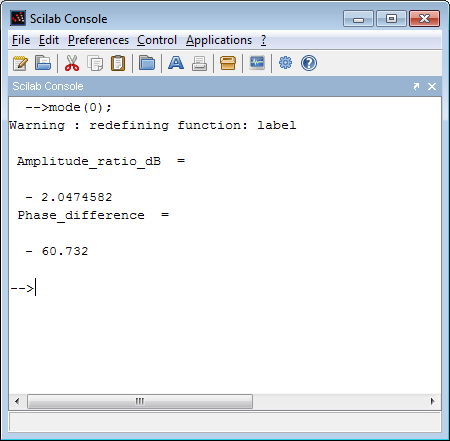
\includegraphics[width=\linewidth]{sinetest_manual/bode_calc.png}
\caption{Scilab Output}
\label{scilab_op}
\end{figure}
It could be seen from figure \ref{scilab_op} that the Amplitude Ratio turns out to be $-2.047$dB and phase difference to be $-60.732$\textdegree.
The plot thus obtained is shown in figure \ref{plot0.4}
\begin{figure}
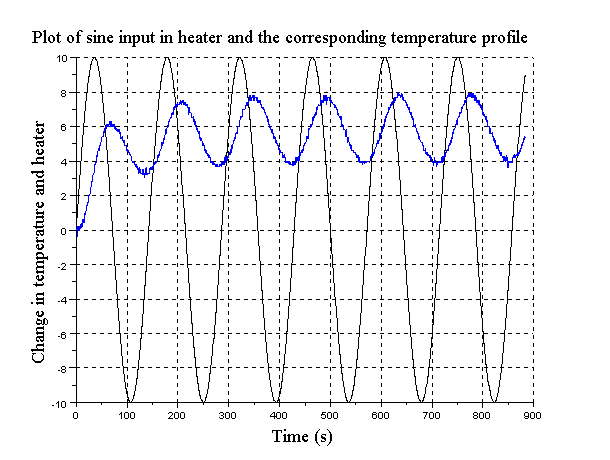
\includegraphics[width=\linewidth]{sinetest_manual/bode_resp}
\caption{Plot of Input and Output vs time}
\label{plot0.4}
\end{figure}

Repeat this calculation over a range of frequencies and note down the values of Amplitude Ratio in dB and Phase Difference. Input these values for the appropriate frequencies in to the Scilab code {\ttfamily BodePlot.sce} and execute it to get a Bode Plot of the plant which is illustrated in figure \ref{bode_plot}.
\begin{figure}
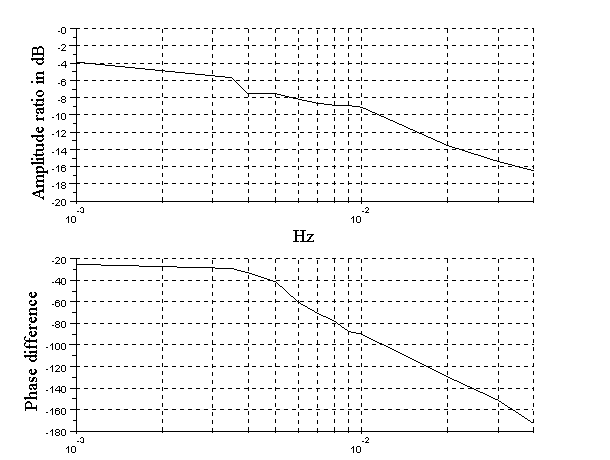
\includegraphics[width=\linewidth]{sinetest_manual/bodeplot}
\caption{Bode Plot obtained from the plant}
\label{bode_plot}
\end{figure}

Bode Plot can be obtained directly from the plants Secon order Transfer function \cite{kmm09} with the help of scilab code {\ttfamily TFbode.sce}, as shown in figure \ref{tfbode}. A visual comparison of the two bode plots can be done to validate the bode diagram obtained from the plant.
\begin{figure}
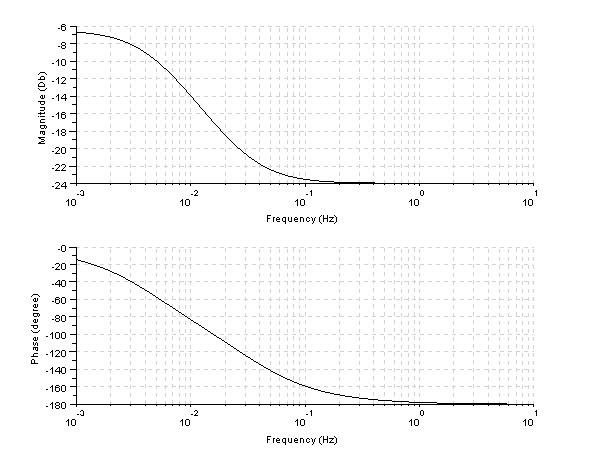
\includegraphics[width=\linewidth]{sinetest_manual/plant_bode_tf}
\caption{Bode Plot obtained through plants Transfer function}
\label{tfbode}
\end{figure}

For comparing above two plots we are plotting it on same graph as shown in figure \ref{compare_bode}
\begin{figure}
\centering
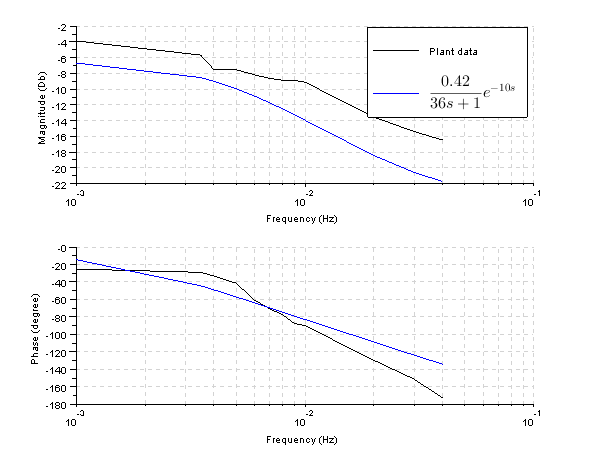
\includegraphics[width=\linewidth]{sinetest_manual/bode_comparison}
\caption{Comparison of Bode Plots}
\label{compare_bode}
\end{figure}


\section{Conducting Sine Test on SBHS, virtually}
The step by step procedure for conducting an experiment virtually is explained in section \ref{vlabsexpt}. The required .sce file is {\tt sinetest.sce}.  You will find this file in the {\tt SineTest} directory under {\tt virtual} folder. Please note that the analysis code of sine test data obtained by a virtual experiment is slightly different. The procedure to use the analysis code however remains the same as explained earlier. To calculate the {\tt Amplitude Ratio} and {\tt Phase Difference}, one has to use the file {\tt sine2\_virtual.sce}. These files are available in the {\tt Sine\_Analysis} folder under the {\tt virtual} folder. The necessary codes are listed in the section \ref{sinecodes}.


\section{Scilab Code}\label{sinecodes}

\begin{code}
\ccaption{sine\_test.sci}{\ttfamily sine\_test.sci}
\lstinputlisting{Scilab/local/Sine_Test/sine_test.sci}
\end{code}


\begin{code}
\ccaption{sinetest.sce}{\ttfamily sinetest.sce}
\lstinputlisting{Scilab/virtual/SineTest/sinetest.sce}
\end{code}

\begin{code}
\ccaption{sinetest.sci}{\ttfamily sinetest.sci}
\lstinputlisting{Scilab/virtual/SineTest/sinetest.sci}
\end{code}

\begin{code}
\ccaption{sine2.sce}{\ttfamily sine2.sce}
\lstinputlisting{Scilab/local/Sine_Analysis/sine2.sce}
\end{code}

\begin{code}
\ccaption{lable.sci}{\ttfamily label.sci}
\lstinputlisting{Scilab/local/Sine_Analysis/label.sci}
\end{code}

\begin{code}
\ccaption{bodeplot.sce}{\ttfamily bodeplot.sce}
\lstinputlisting{Scilab/local/Sine_Analysis/bodeplot.sce}
\end{code}


\begin{code}
\ccaption{labelbode.sci}{\ttfamily labelbode.sci}
\lstinputlisting{Scilab/local/Sine_Analysis/labelbode.sci}
\end{code}


\begin{code}
\ccaption{TFbode.sce}{\ttfamily TFbode.sce}
\lstinputlisting{Scilab/local/Sine_Analysis/TFbode.sce}
\end{code}

\begin{code}
\ccaption{comparison.sce}{\ttfamily comparison.sce}
\lstinputlisting{Scilab/local/Sine_Analysis/comparison.sce}
\end{code}

\begin{code}
\ccaption{sine2\_virtual.sce}{\ttfamily sine2\_virtual.sce}
\lstinputlisting{Scilab/virtual/Sine_Analysis/sine2_virtual.sce}
\end{code}

